\clearpage
\appendix


\section{Network Architecture}

The network architecture of \nameMethod is depicted in \cref{fig:architecture}. 
The newly introduced animation-time embedder $\mathcal{E}_{\text{ani}}$ encodes the source and target animation times, $\animatime_\src$ and $\animatime_\trg$, into tensors matching the shapes of $x_\src$ and $x_\trg$, which are then added to them respectively.
During training, we train only the camera embedder $\mathcal{E}_{\text{cam}}$, the animation-time embedder $\mathcal{E}_{\text{ani}}$, the self-attention (full-3D attention), and the projector layers before the cross-attention.
\begin{figure}[h]
    \centering
    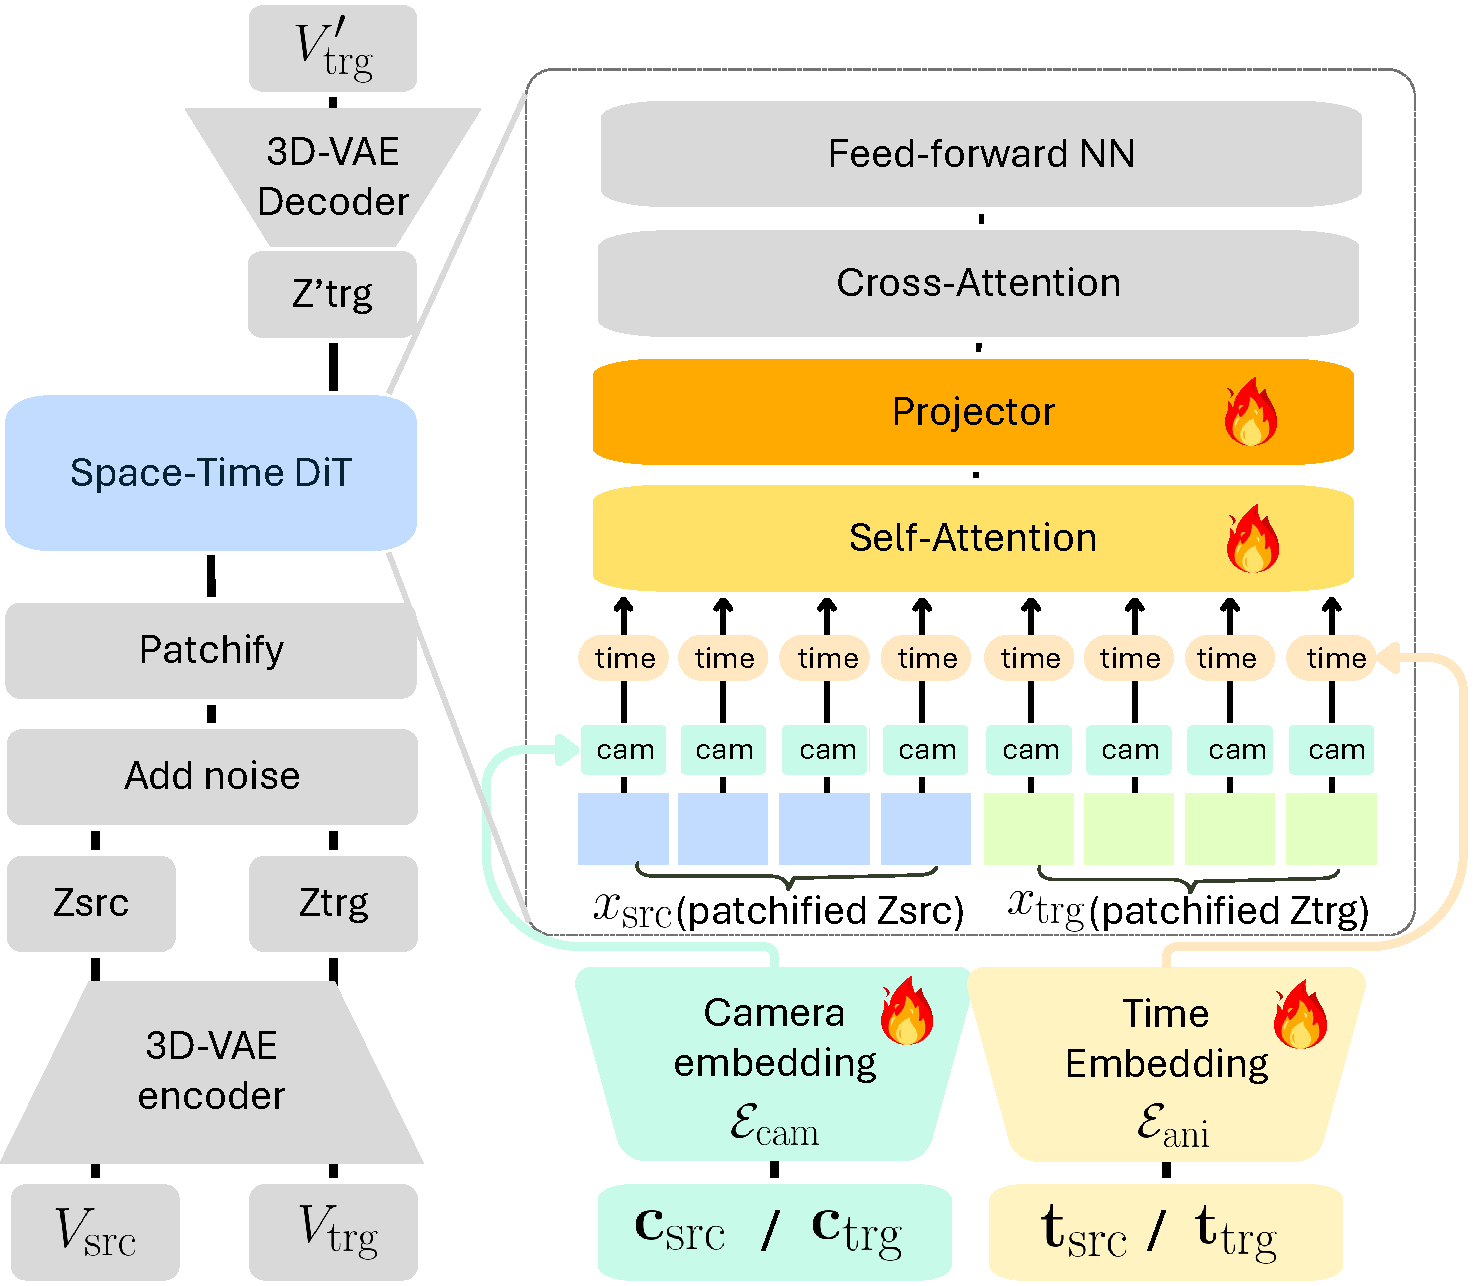
\includegraphics[width=\linewidth]{figures/src_files/architecture.pdf}
    \caption{
        \textbf{Architecture of \nameMethod.}
        Our model jointly conditions on camera trajectories and temporal control signals via space–time attention, enabling non-monotonic motion generation such as reversals, repeats, accelerations, and zigzag time.}
    \label{fig:architecture}
\end{figure}


\begin{figure*}[t]
    \centering
    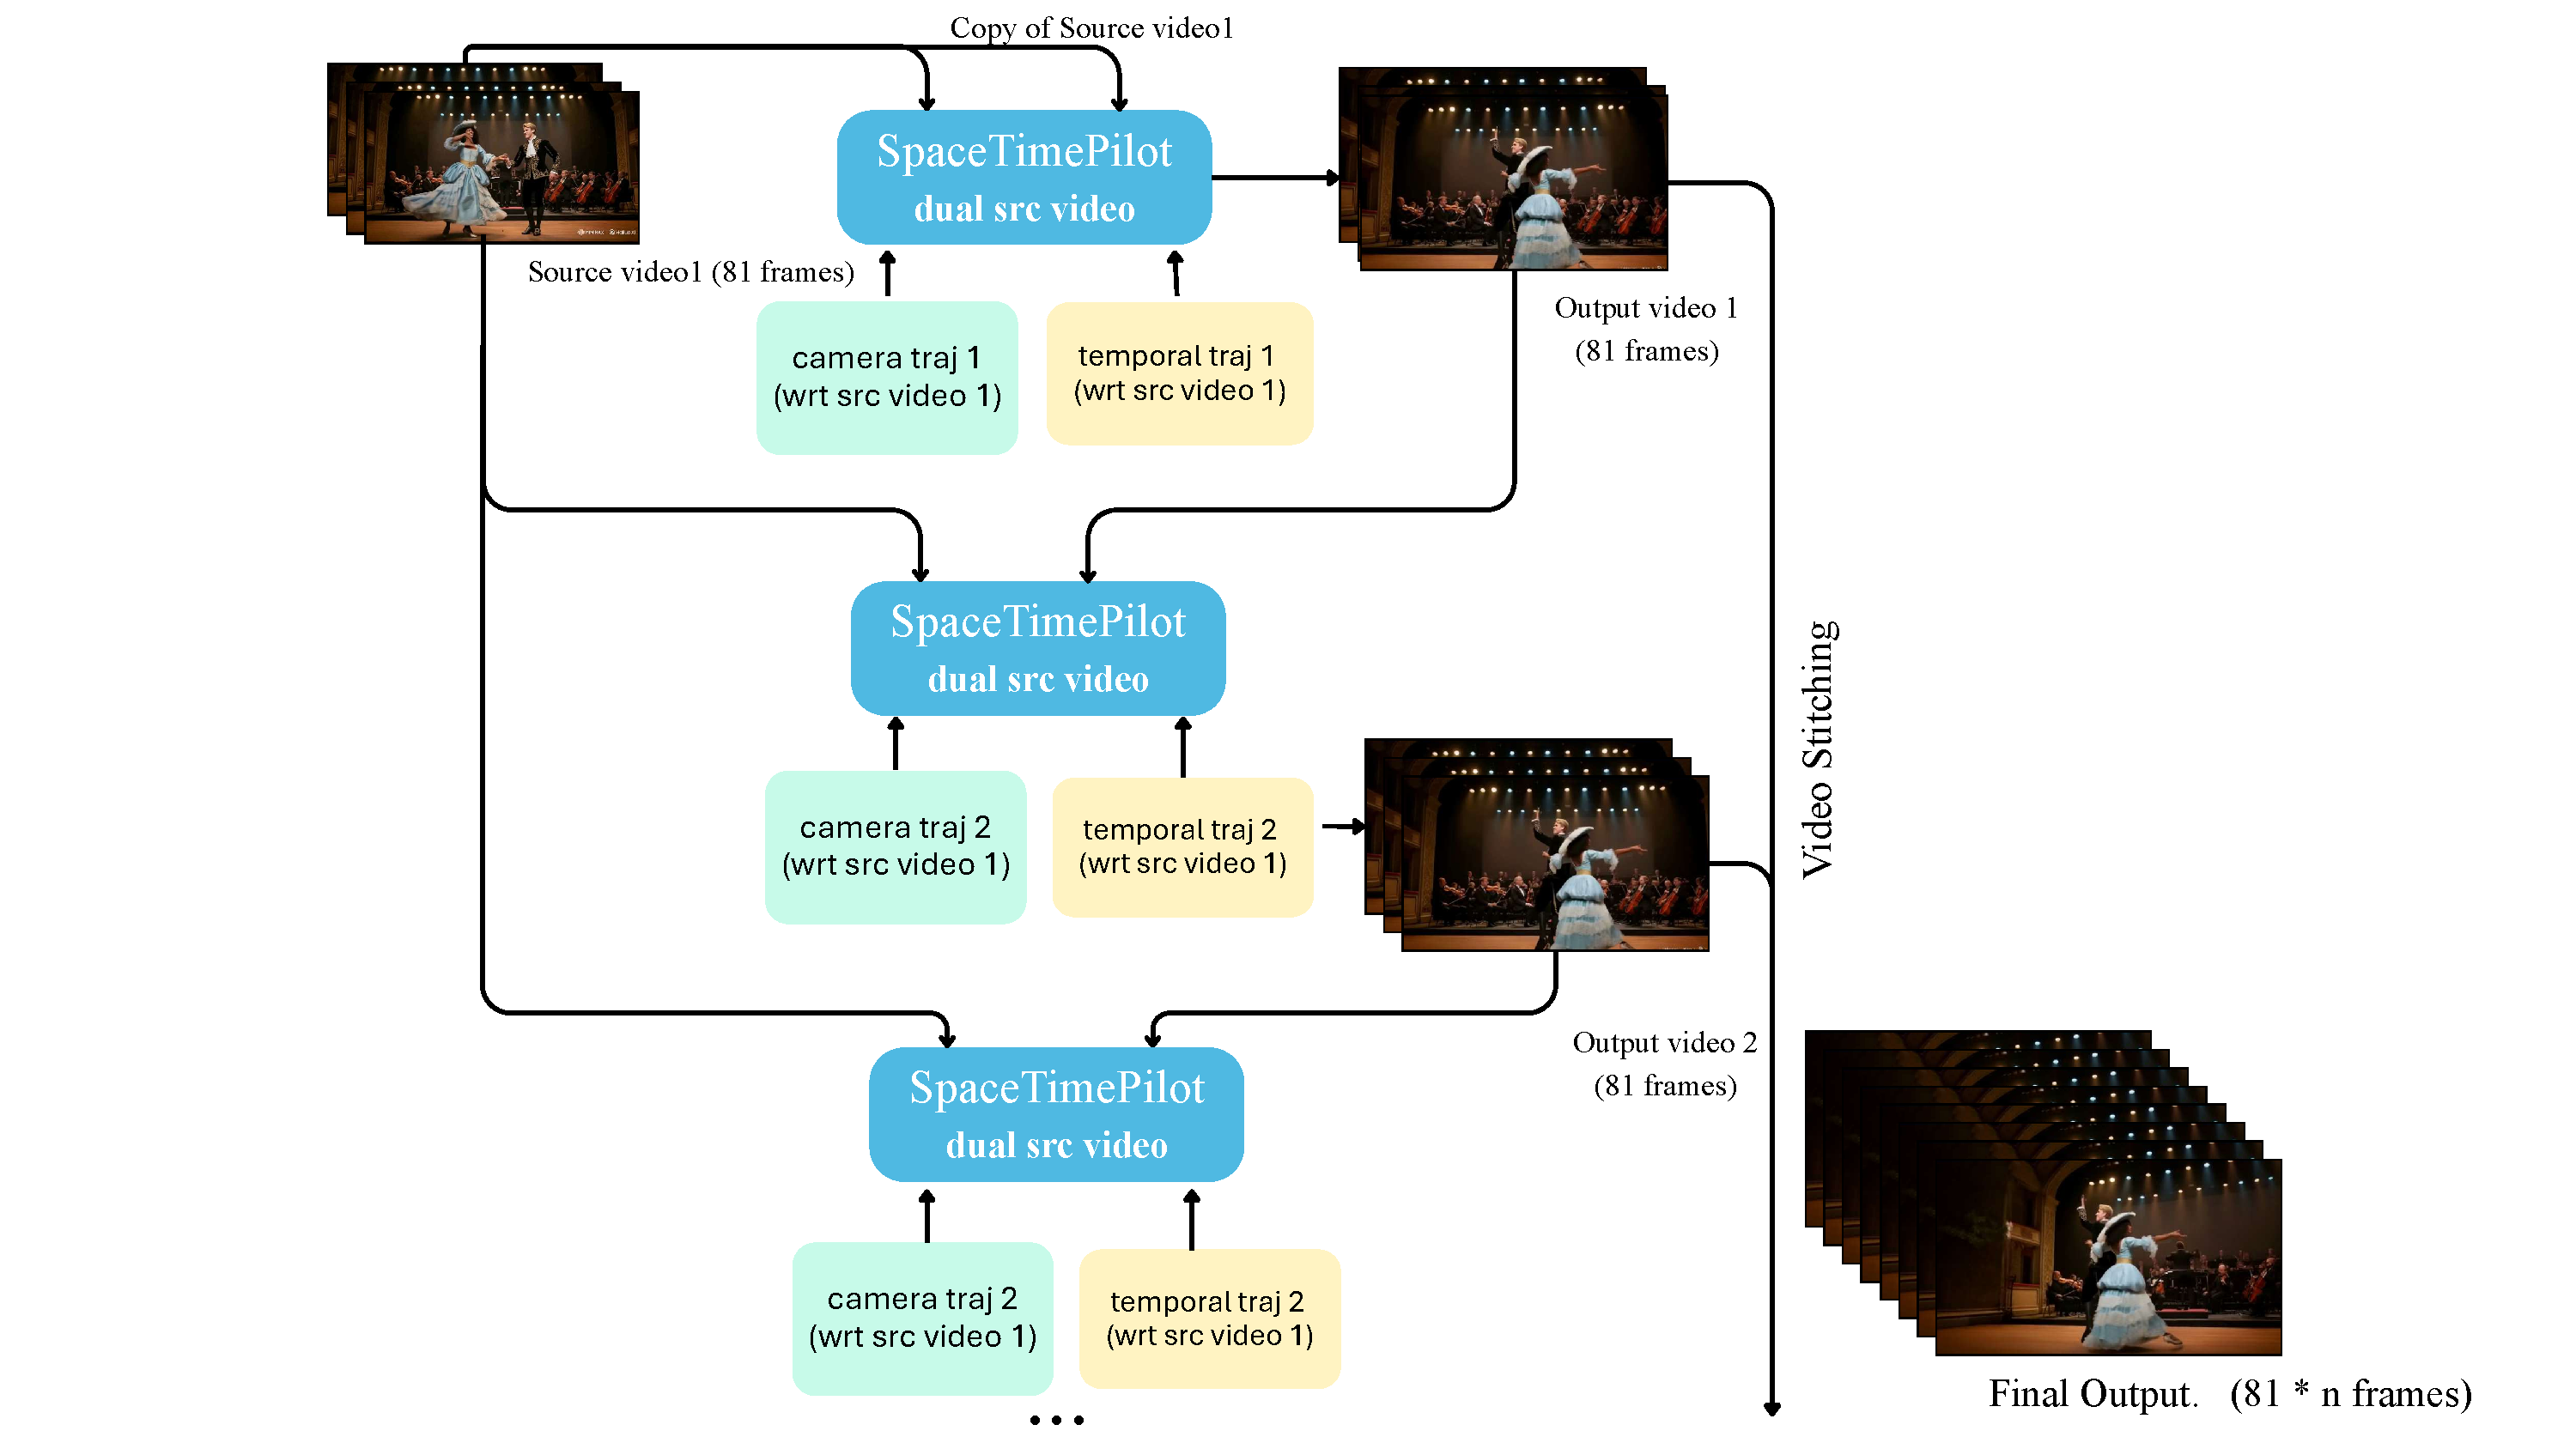
\includegraphics[width=\linewidth]{figures/AR-pipeline.pdf}
    \caption{
        \textbf{Overview of the multi-turn autoregressive inference scheme.}
The model first generates an 81-frame segment conditioned on the source video and a chosen space–time trajectory. The resulting output is then reused as a secondary source video for subsequent iterations, each with its own camera and temporal trajectory. By chaining these iterations and stitching the outputs, \nameMethod produces a long, coherent video that follows an arbitrary space–time path.
    }
    \label{fig:multi-turn}
\end{figure*}

\section{Longer Space-Time Exploration Video with Disentangled Controls}

 One of the central advantages of \nameMethod is its ability to freely navigate both spatial and temporal dimensions, with arbitrary starting points in each dimension and fully customizable trajectories through them. Although each individual generation is limited to an 81-frame window, we show that \nameMethod can effectively extend this window indefinitely through a multi-turn autoregressive inference scheme, enabling continuous and controllable space–time exploration from a single input video. The overall pipeline is illustrated in \cref{fig:multi-turn}.

The core idea is to generate the final video in autoregressive segments that connect seamlessly.  For example, given a source video of 81 frames, we may first generate a 0.5$\times$ slow-motion sequence covering frames 0–40 with a new camera trajectory. Then, continuing both the visual context and the generated camera trajectory, we can produce the next segment starting from the final camera pose of the previous output, while temporally traversing the remaining frames 40–81. This yields an autoregressive chain of viewpoint-controlled video segments that together create a continuous long-range space–time trajectory.

A key property that enables this behavior is that our model can generate video segments whose camera poses do \emph{not} need to start at the first frame. 
This allows precise control over the starting point, both in time and viewpoint, for every generated chunk, ensuring smooth, consistent motion over extended sequences.

To maintain contextual coherence across iterations, we introduce a lightweight memory mechanism. During training, the model is conditioned on \textbf{a pair of source videos}, which enables consistent chaining during inference. Specifically:
\begin{itemize}
\item At iteration $i = 1$, the model is conditioned only on the original source video.
\item At iteration $i = 2$, it is conditioned on both the source video and the previously generated 81-frame segment.
\item This process repeats, with each iteration conditioning on the source video as well as the most recent generated segment.
\end{itemize}

This simple yet effective strategy allows \nameMethod to generate arbitrarily long, smoothly connected sequences with continuous and precise control over both temporal manipulation and camera motion.

Here, we showcase how this can be used to conduct large viewpoint changes, as demonstrated in \cref{fig:multi-turn demo}.



\begin{figure*}[t]
    \vspace{-5mm}
    \centering
    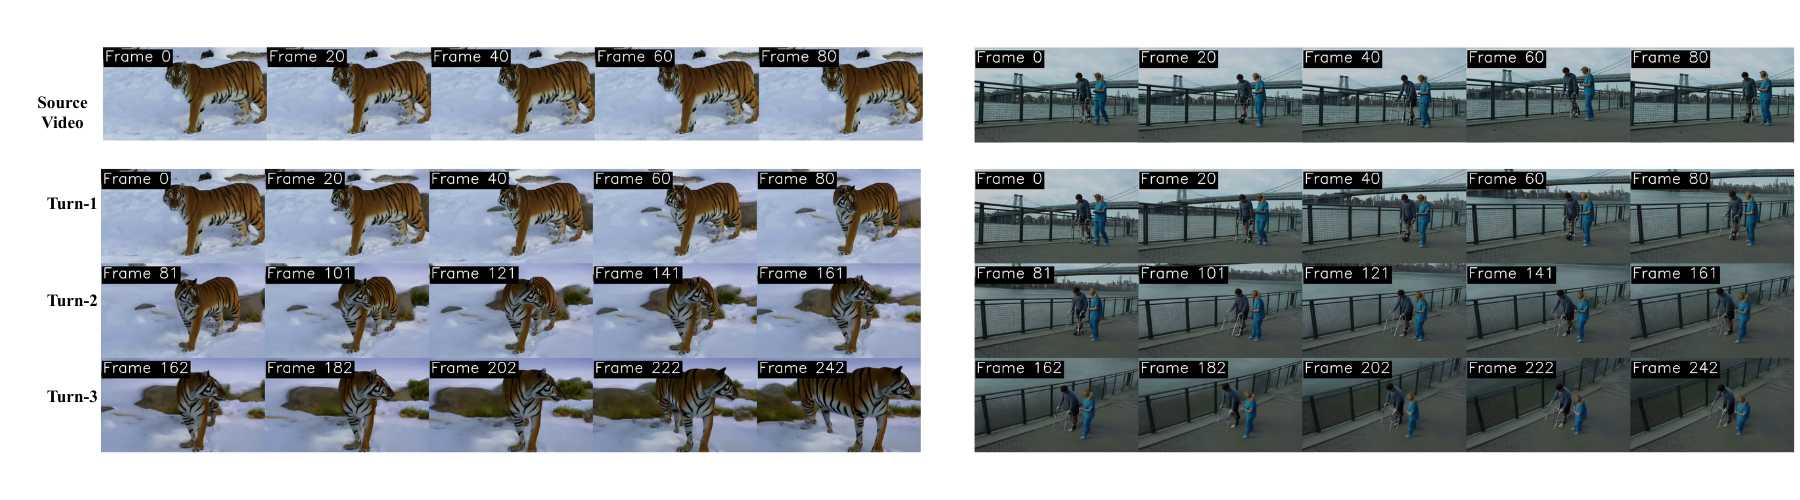
\includegraphics[width=\linewidth]{figures/src_files/ar_demo.jpg}
    \vspace{-1Cm}
    \caption{
       \textbf{ Multi-turn autoregressive generation with \nameMethod.} Top row: source video frames.
Rows 2–4: Turn-1, Turn-2, and Turn-3 generations.
At each turn, \nameMethod jointly conditions on (1) the original source video and (2) the previously generated chunk, ensuring temporal continuity, stable motion progression, and consistent camera geometry.
This dual-conditioning design enables viewpoint changes far beyond the input video—such as rotating to the rear of the tiger or transitioning from a low-angle shot to a high bird’s-eye view—while preserving visual and motion coherence. Please refer to section ``AR Demos'' in the website for videos.
    }
    \label{fig:multi-turn demo}
\end{figure*}




\section{Additional Details on the Proposed \nameDataset Dataset.}

The \texttt{\nameDataset} dataset is built using high-quality, commercially licensed 3D environments that include both realistic indoor and outdoor scenes. For each environment, we populate the space with multiple animated human characters. 
The character assets are sourced from Mixamo \cite{mixamo} and HUMOTO \cite{Lu_2025_HUMOTO}, and each character is manually textured and refined to ensure realistic geometry, appearance, and material quality. 
The animations span a diverse range of human motions, including locomotion, gestures, and human-object interactions.
Examples of scenes are shown in \cref{fig:visualexample}. 
Please refer to the complementary website for the video examples.

To capture rich spatial coverage, we generate four distinct camera trajectories for every scene. Camera paths include rotational orbits, linear tracking motions, and smoothly curved arcs. A dedicated validity module ensures that each trajectory:
(1) begins at a collision-free location with clear visibility of the main character,
(2) maintains non-intersecting movement with the environment throughout the path, and
(3) preserves full subject visibility across all viewpoints.

Each trajectory is rendered into a 120-frame sequence at a resolution of $1080 \times 1080$ pixels, providing dense temporal sampling with high visual fidelity. This yields three multi-view video sequences per scene, each covering the full motion duration with consistent lighting, textures, and geometry. Overall, we rendered 1500 videos from 500 animations, each with 120 videos full grid rendering, leading to 180k videos.

For temporal-control training, we could sample any time variants from these sequences, including slow motion, reverse playback, bullet-time around arbitrary frames, and non-monotonic time patterns such as forward–backward oscillation. These augmented temporal signals are illustrated in \cref{fig:sampling}.

\begin{figure}[ht]
    \centering
    \vspace{-3mm}
    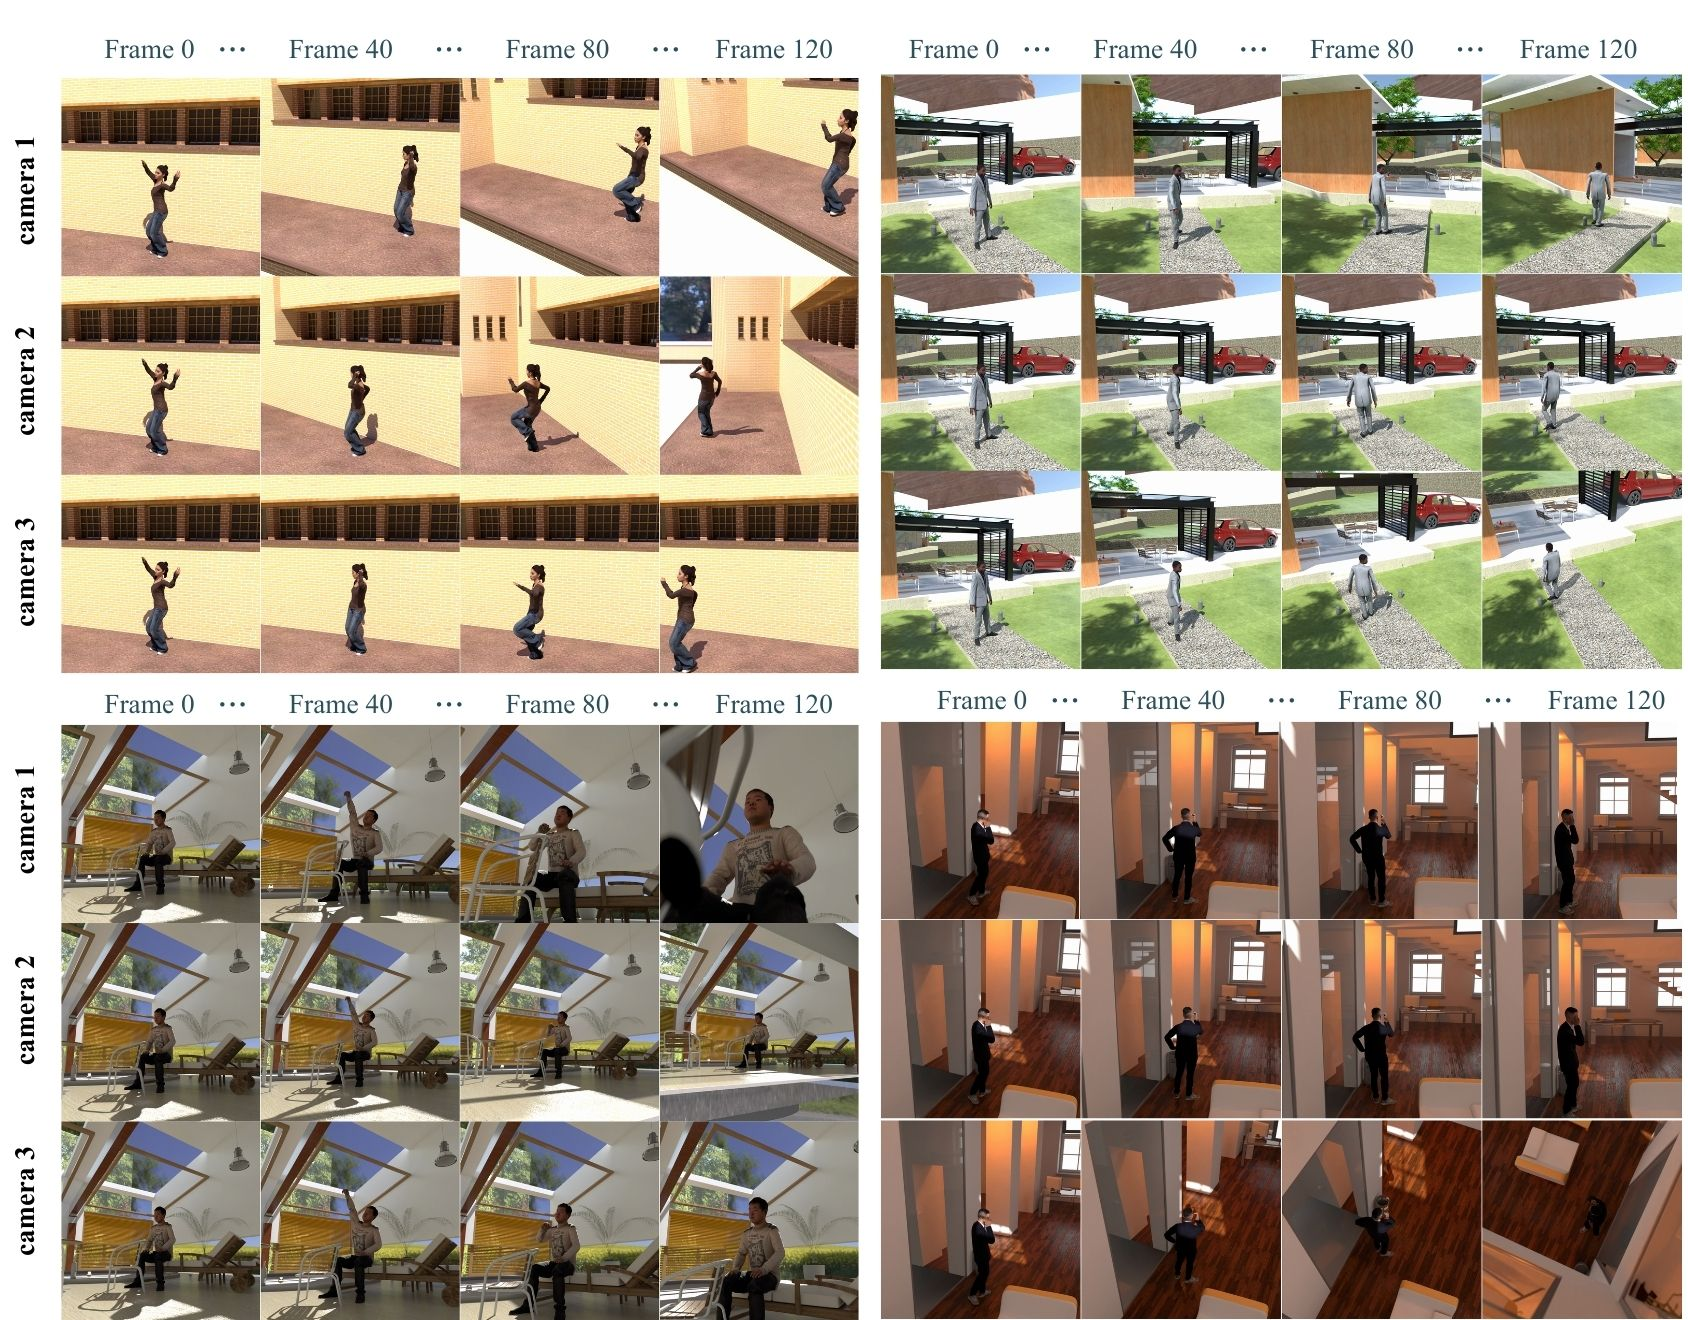
\includegraphics[width=\linewidth]{figures/src_files/data_demo.jpg}
    \caption{\textbf{Example of \nameDataset}.
   Multi-view, densely sampled sequences from the \nameDataset dataset. Each row shows frames from one camera trajectory, and each column samples different timesteps (0–120). The dataset provides diverse environments, human motions, and four camera paths per scene with full 120-frame temporal coverage.
    }
    \label{fig:visualexample}
\end{figure}

\begin{figure}[ht]
    \centering
    \vspace{-3mm}
    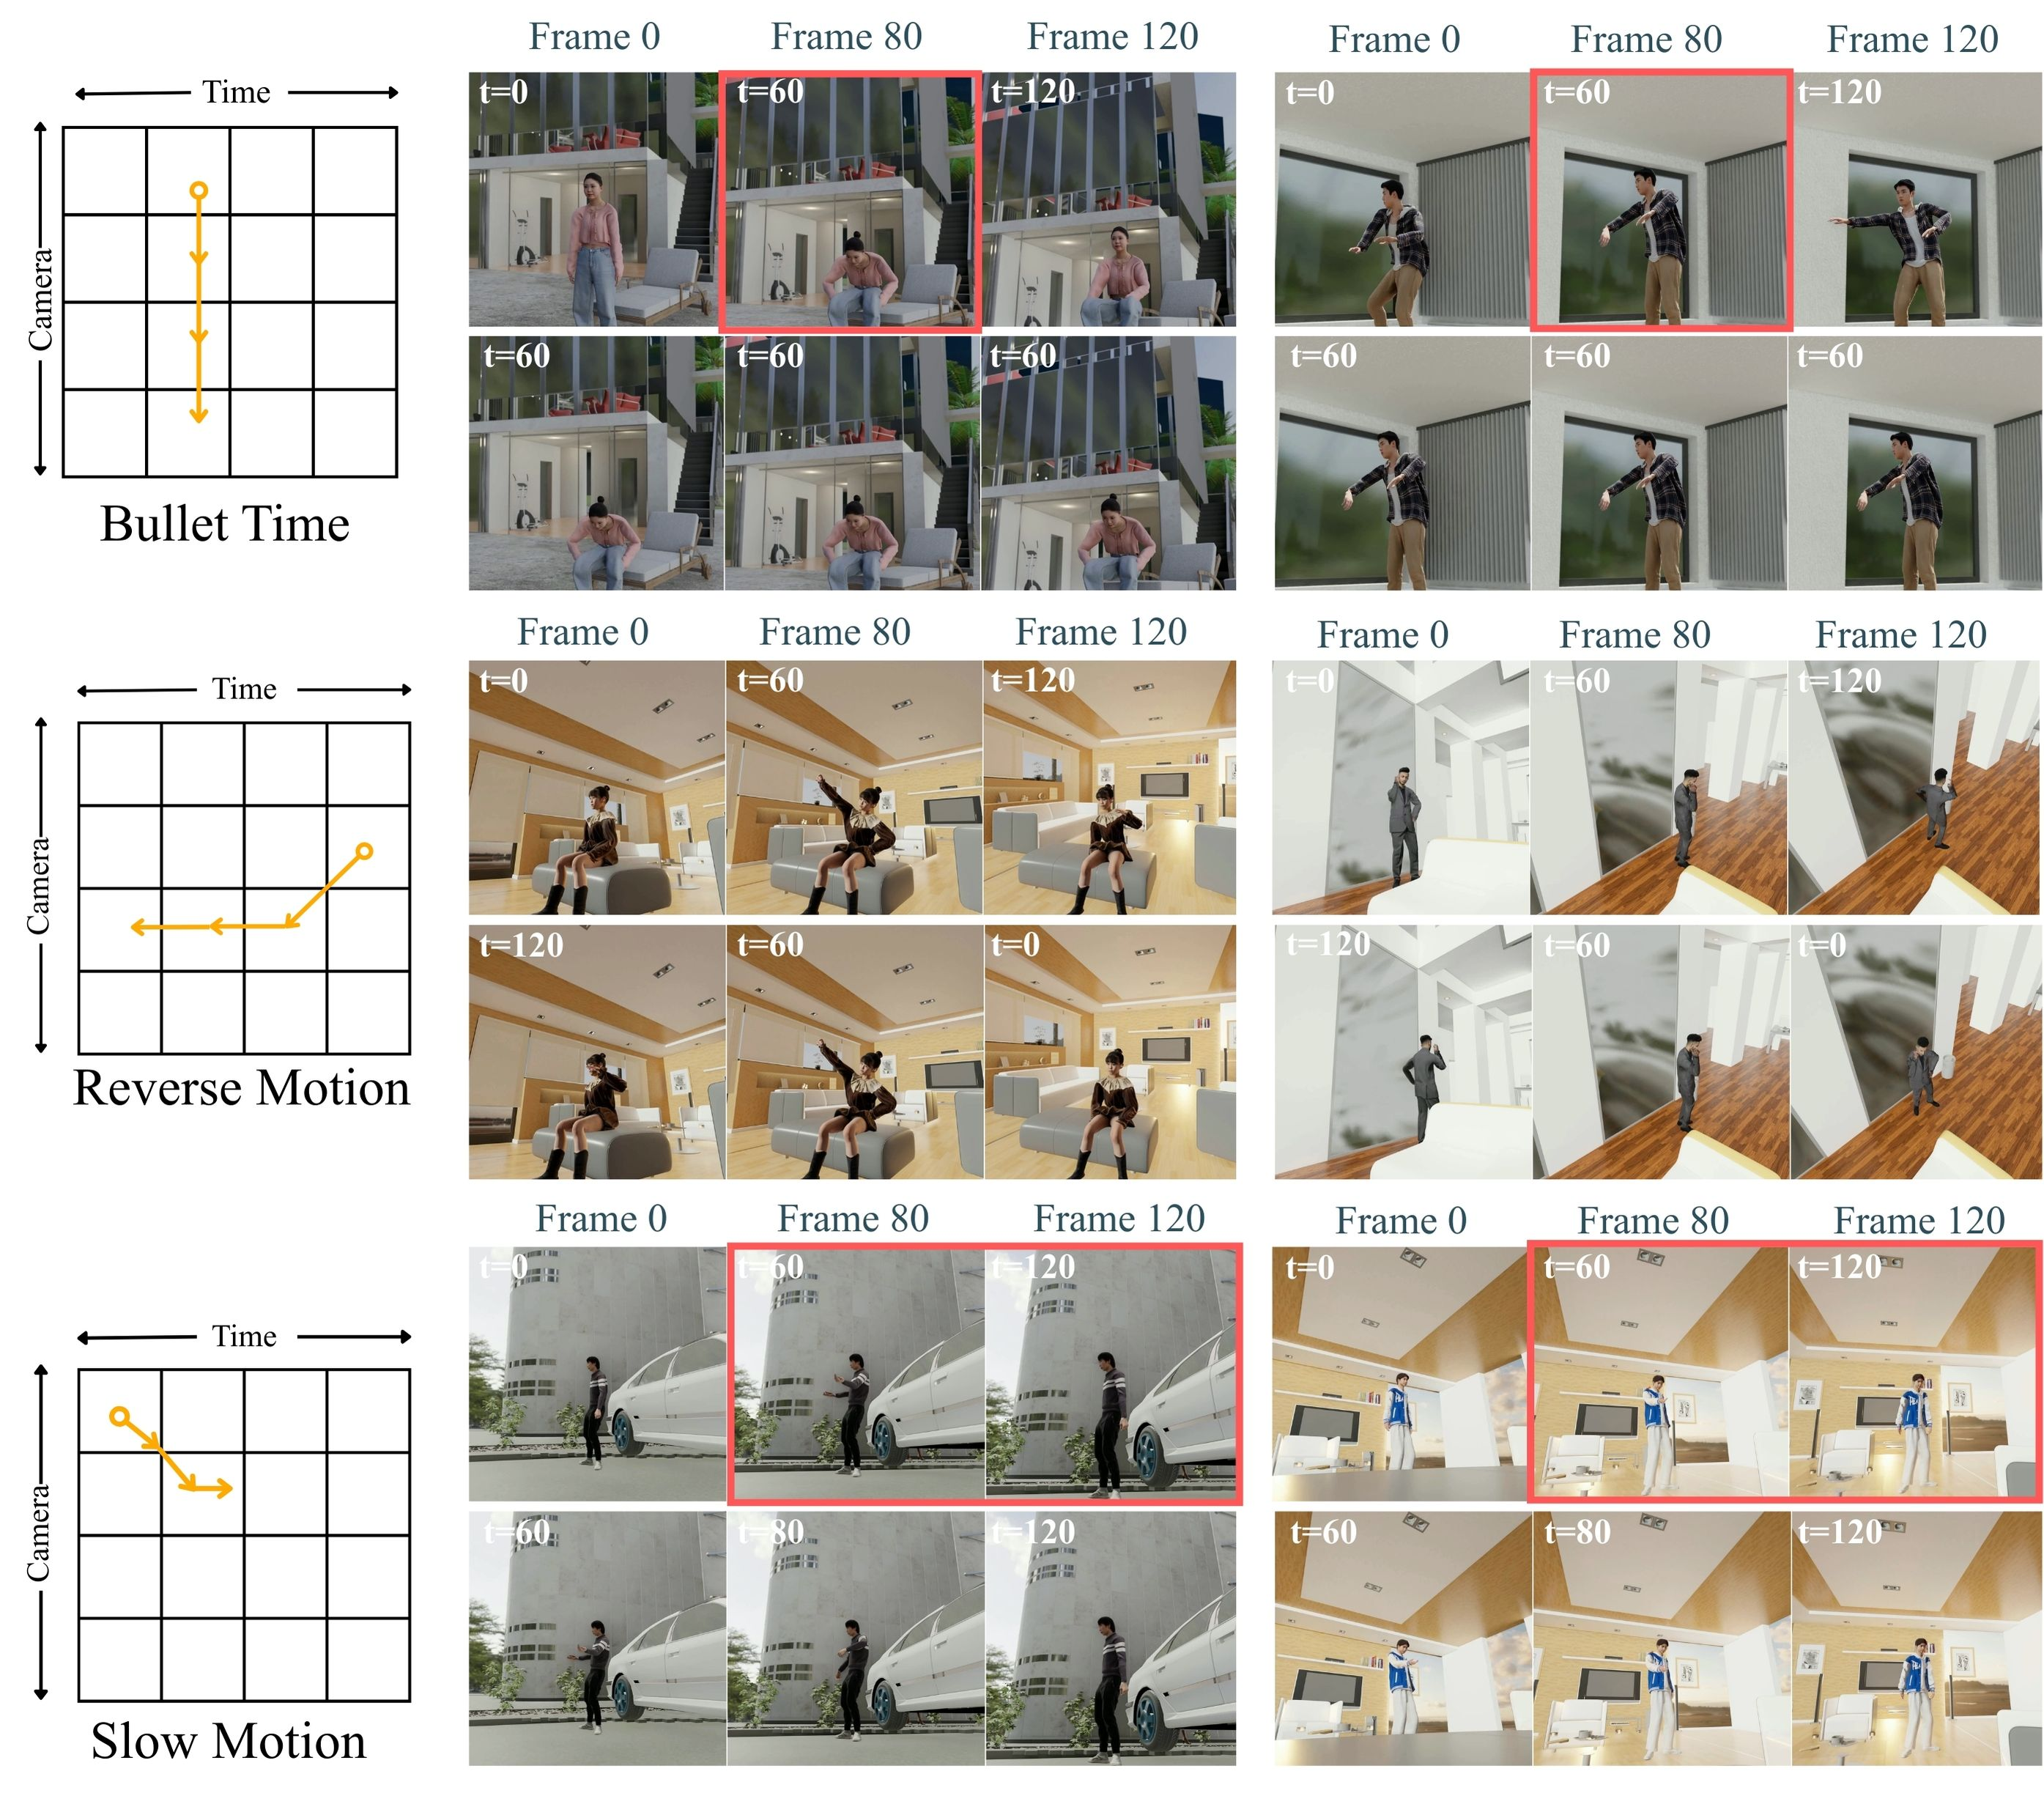
\includegraphics[width=\linewidth]{figures/src_files/sampling_example.jpg}
    
    \caption{
    \textbf{Sampling from \nameDataset.}
By sampling from the \nameDataset dataset, we can extract frames corresponding to arbitrary combinations of camera viewpoints and temporal positions, forming source-target pairs with rich camera and temporal control signals.
    }
    \label{fig:sampling}
\end{figure}

\begin{figure*}[ht]
    \centering
    \vspace{-3mm}
    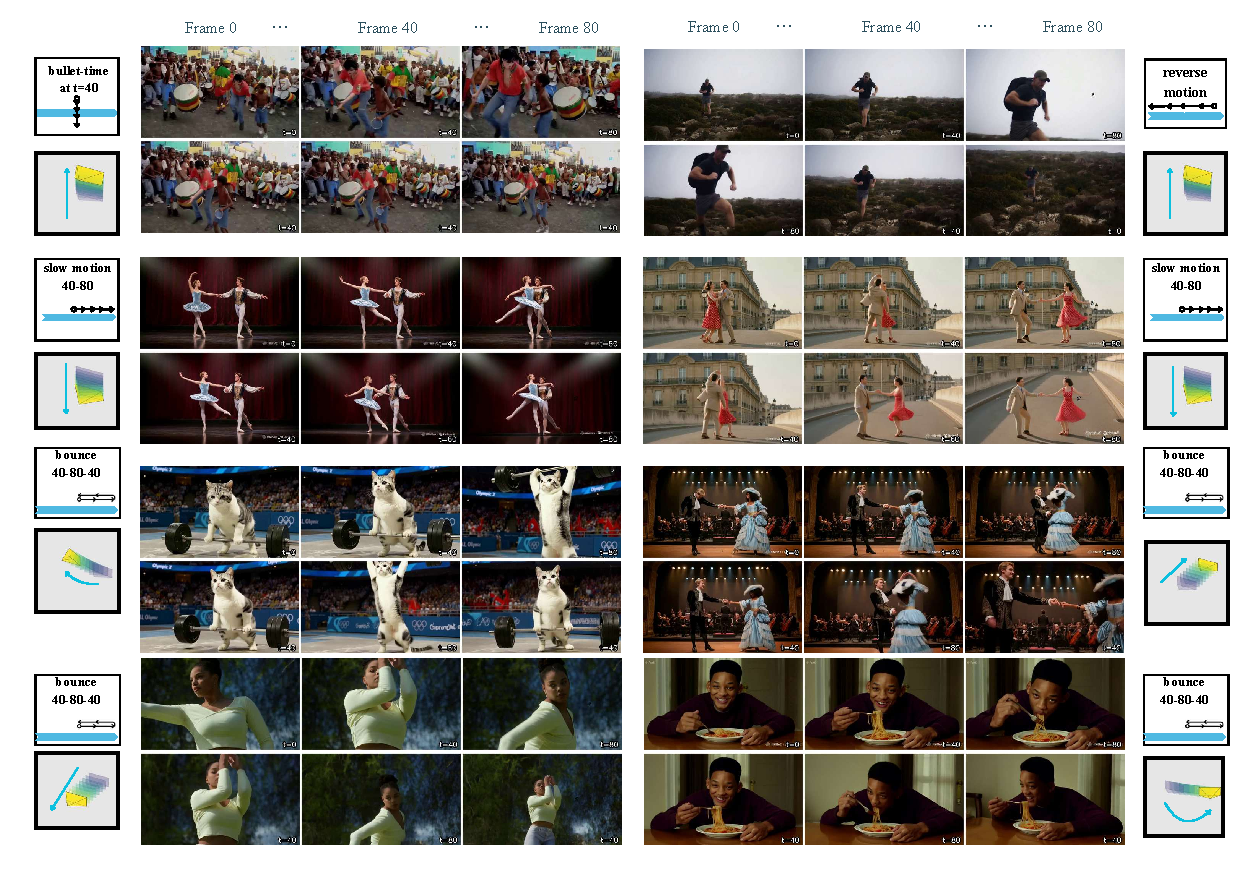
\includegraphics[width=\linewidth]{figures/more_results.pdf}
    \caption{
    \textbf{More Qualitative results.}
Our model provides fully disentangled control over camera motion and temporal dynamics. Each row illustrates a different combination of temporal control inputs (top-left icon) and camera trajectories. \nameMethod consistently produces coherent videos across a wide range of controls, including normal and reverse playback, bullet-time, slow motion, replay motion, and complex camera paths such as panning, tilting, zooming, and vertical motion.
    }
    \label{fig:more_quali}
\end{figure*}




\section{Additional Ablation Studies}

\subsection{Temporal Warping Augmentation}
\begin{figure*}[ht]
    \centering
    \vspace{-3mm}
    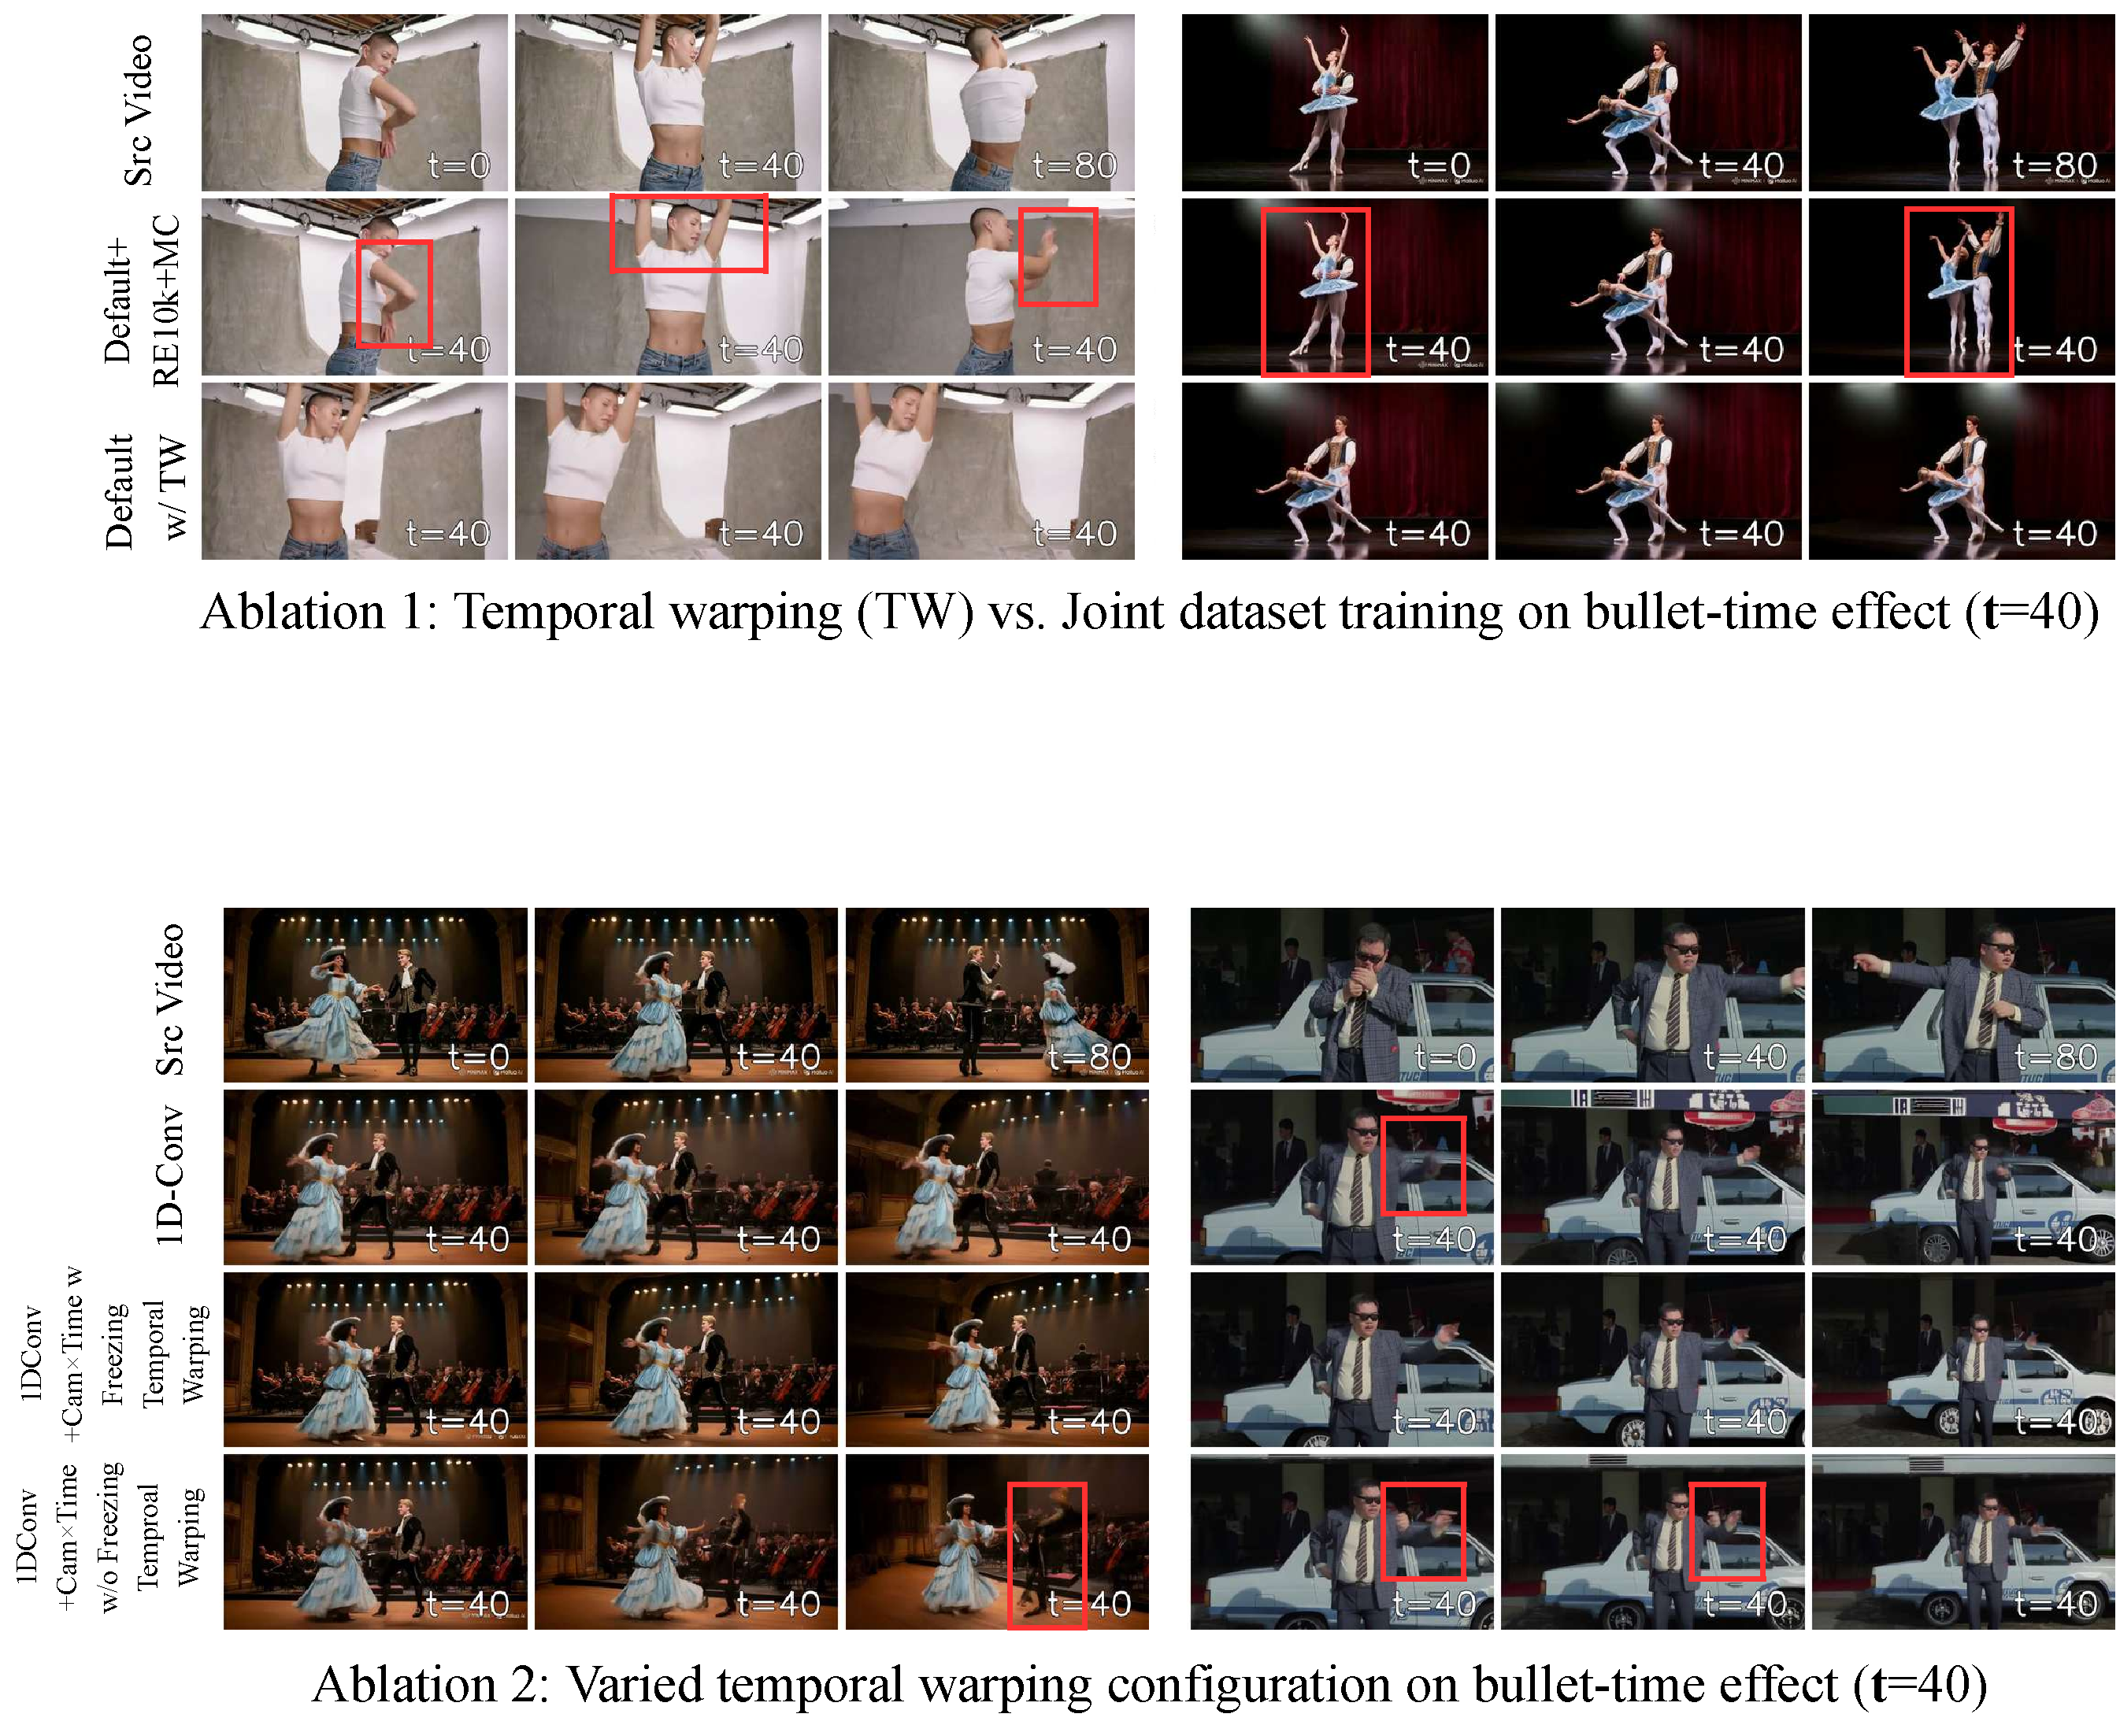
\includegraphics[width=\linewidth]{figures/src_files/ablation_1_2.pdf}
    
    \caption{
    \textbf{Ablation study.}
    (Top) Using \cite{Bai2025,bai2024syncammaster} as default datasets, we compare the influence of adding static-scene datasets \cite{zhou2018stereo,li2019mannequin} vs.~just doing temporal warping (TW) augmentation (Sec.~3.2.2 in the main paper). Temporal warping definitely provide more variety of time control signals, allowing models to learn better camera-time disentanglement. 
    (Bottom) We further compare different configurations of warping, where we show freezing temporal warping (3\textsuperscript{rd} row) leads to better results than those trained without freezing temporal warping.
    }
    \label{fig:ablation_1_2}
\end{figure*}

Using \cite{Bai2025,bai2024syncammaster} as our default datasets, we compare training jointly with static-scene datasets \cite{zhou2018stereo,li2019mannequin} with applying only temporal warping (TW) augmentation on the default datasets (Sec.~3.2.2 in the main paper). Although static-scene datasets naturally support bullet-time effects, they do not provide enough diversity of temporal control configurations for models to reliably learn time locking on their own, as shown in \cref{fig:ablation_1_2} (top). Please refer to section ``Effective Temporal Warping'' in the website for more videos.

In \cref{fig:ablation_1_2} (bottom), we further show that freezing temporal warping (3rd row) produces better results than training without freezing it. Please refer to section ``Freeze Warping Ablations'' in the website for more videos. 

\subsection{Significance of \texttt{\nameDataset} Dataset}
Besides the quantitative results in the main paper (Table 5), in \cref{fig:ablation_3_4} (top), we provide visual comparisons demonstrating the effectiveness of the proposed \texttt{\nameDataset} dataset. 
Clear artifacts appear in baselines trained without additional data or with only static-scene augmentation (highlighted in red boxes), whereas incorporating \texttt{\nameDataset} removes these artifacts, demonstrating its significance. Please refer to section ``Dataset Ablations'' in the website for more videos.

\subsection{Time Embedding Ablation}
\begin{figure*}[ht]
    \centering
    \vspace{-3mm}
    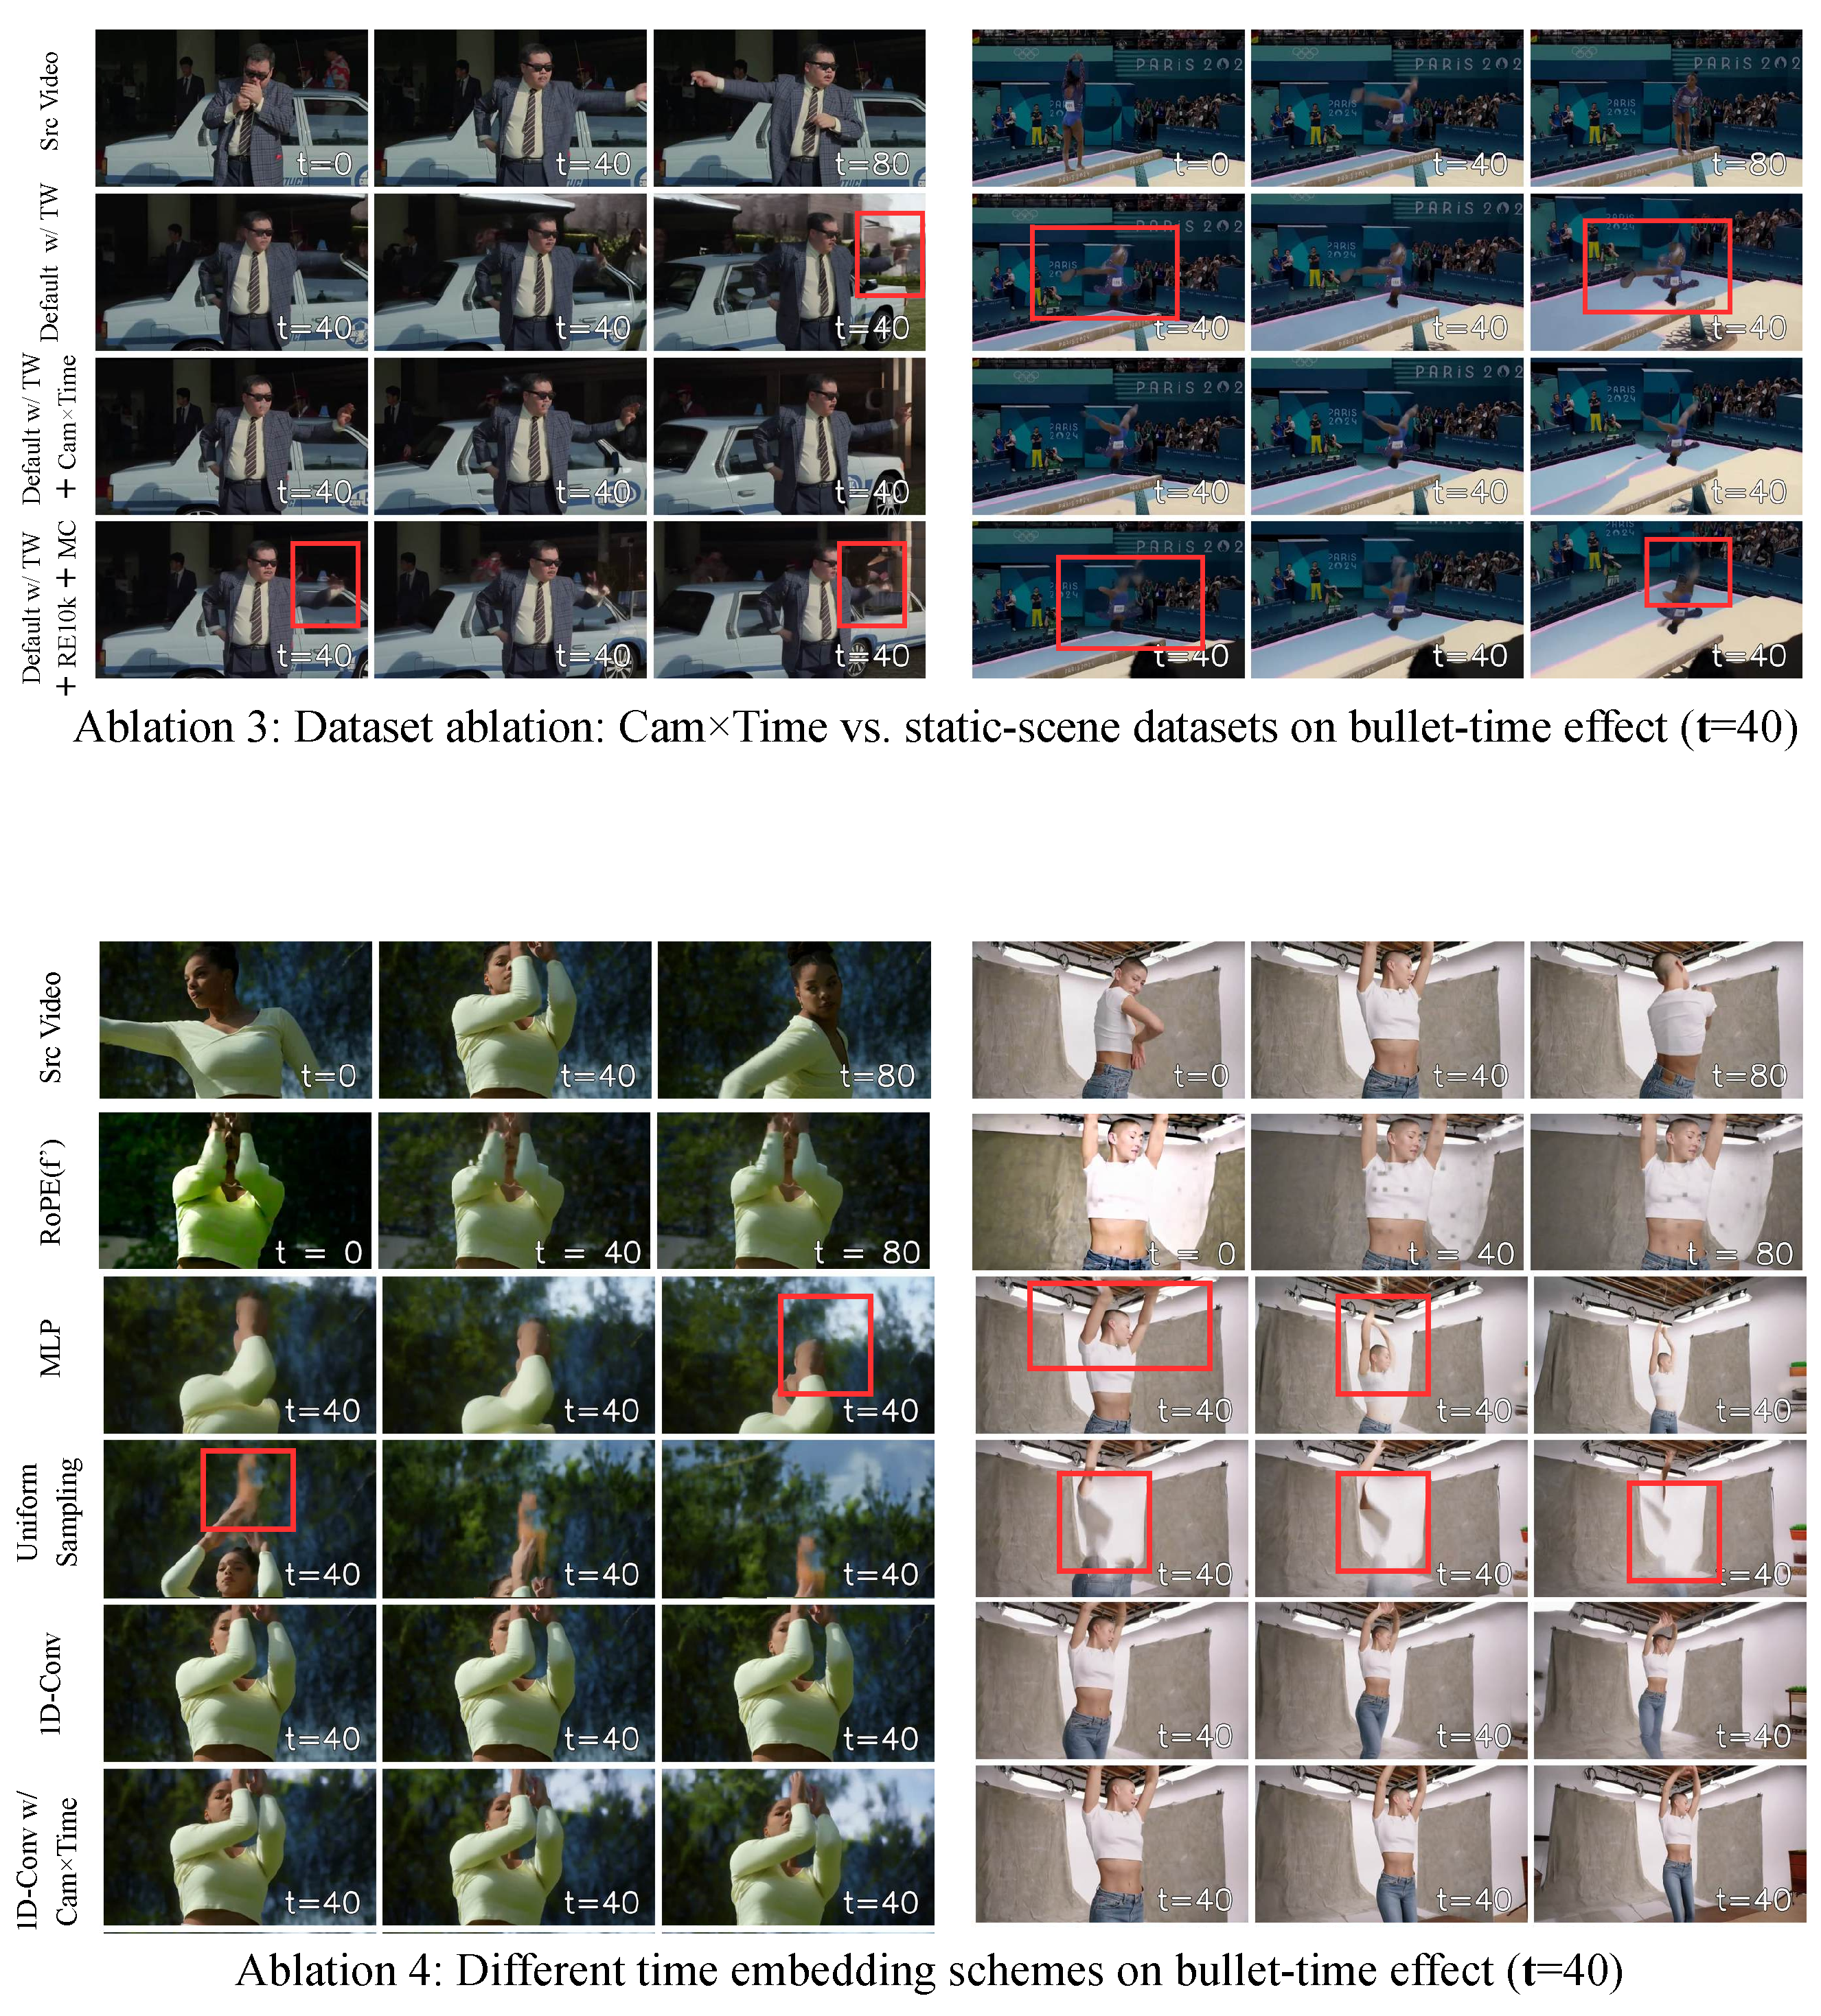
\includegraphics[width=\linewidth]{figures/src_files/ablation_3_4.pdf}
    
    \caption{
    \textbf{Ablation study.}
    (Top) We verify the efficacy of the proposed \nameDataset dataset. Considering \cite{Bai2025,bai2024syncammaster} as default datasets, we compare the impact of different datasets on the generated videos. One can clearly see artifacts in baselines without any extra data or augmented with static-scene data, whereas training additionally with \nameDataset leads to no artifacts, confirming the usefulness of our dataset.
    (Bottom) We compare several time-embedding strategies. The MLP fails to lock the temporal state (red boxes), while RoPE($f'$) correctly freezes the scene dynamics at $\animatime$=40 but unintentionally locks the camera motion too. Conditioning on the latent frame $f'$ (with uniform sampling) introduces noticeable artifacts. In contrast, the proposed 1D-Conv embedding allows \nameMethod to both freeze the scene dynamics at $\animatime$=40 and produce intended camera motion. Incorporating \nameDataset during training further improves performance.
    }
    \label{fig:ablation_3_4}
\end{figure*}

As promised in Sec.~3.2.1 in the main paper, we compare several time-embedding strategies. RoPE($f'$) can freeze the scene dynamics at $\animatime$=40, but it also undesirably locks the camera motion. 
Using MLP, by contrast, fails to lock the temporal state at all (red boxes).
Conditioning on the latent frame $f'$ (with uniform sampling) introduces noticeable artifacts. 
In comparison, the proposed 1D-Conv embedding enables \nameMethod to preserve the intended scene dynamics while still generating accurate camera motion. Adding \texttt{\nameDataset} to training further enhances the results. Please refer to section ``Time-Embedding Method Ablation'' in the website for more examples.

\section{Additional Qualitative Visualizations}
We show more qualitative results of \nameMethod in \cref{fig:more_quali}.
Our model provides fully disentangled control over camera motion and temporal dynamics. Each row presents a different pairing of temporal control inputs (top-left icon) and camera trajectories. \nameMethod reliably generates coherent videos under diverse conditions, including normal and reverse playback, bullet-time, slow motion, replay motion, and complex camera movements such as panning, tilting, zooming, and vertical translation. Please refer to section ``Video Demonstrations'' in the website for more examples. 

\clearpage
